\documentclass{article}
\usepackage{arxiv}

\usepackage[utf8]{inputenc}
\usepackage[english, russian]{babel}
\usepackage[T1]{fontenc}
\usepackage{url}
\usepackage{booktabs}
\usepackage{amsfonts}
\usepackage{nicefrac}
\usepackage{microtype}
\usepackage{lipsum}
\usepackage{graphicx}
\usepackage{natbib}
\usepackage{doi}



\title{Восстановление прогноза, сделанного в метрическом вероятностном пространстве, в исходное пространство (временных рядов)}

\author{ Maxim Divilkovskiy \\
% \thanks{Use footnote for providing further
% 		information about author (webpage, alternative
% 		address)---\emph{not} for acknowledging funding agencies.} \\
	Chair of Data Analysis\\
	MIPT\\
	% Pittsburgh, PA 15213 \\
	\texttt{divilkovskii.mm@phystech.edu} \\
	%% examples of more authors
	\And
	Vadim Strijov \\
	FRC CSC of the RAS\\
	Moscow, Russia\\
        strijov@phystech.edu \\
	% Santa Narimana, Levand \\
	% \texttt{stariate@ee.mount-sheikh.edu} \\
	%% \AND
	%% Coauthor \\
	%% Affiliation \\
	%% Address \\
	%% \texttt{email} \\
	%% \And
	%% Coauthor \\
	%% Affiliation \\
	%% Address \\
	%% \texttt{email} \\
	%% \And
	%% Coauthor \\
	%% Affiliation \\
	%% Address \\
	%% \texttt{email} \\
}
\date{}

\renewcommand{\shorttitle}{\textit{arXiv} Template}

%%% Add PDF metadata to help others organize their library
%%% Once the PDF is generated, you can check the metadata with
%%% $ pdfinfo template.pdf
\hypersetup{
pdftitle={A template for the arxiv style},
pdfsubject={q-bio.NC, q-bio.QM},
pdfauthor={David S.~Hippocampus, Elias D.~Striatum},
pdfkeywords={First keyword, Second keyword, More},
}

\begin{document}
\maketitle

\begin{abstract}
	Исследование посвящено проблеме прогнозирования временных рядов с высокой ковариацией. Задача решается для наборов временных рядов с высокой дисперсией, проявляющейся, например, в сигналах головного мозга или ценах финансовых активов. Для решения данной задачи предлагается построение пространства парных расстояний, представляющего метрическую конфигурацию временных рядов. Прогноз осуществляется в этом пространстве, а затем результат возвращается в исходное пространство.
	В данной статье рассматриваются методы перевода прогноза из метрического пространства в исходное пространство временных рядов. Помимо этого, приводится оценка качества прогноза. Новизна работы заключается в использовании риманова пространства в качестве метрического, а также в использовании римановых моделей.


\end{abstract}


\keywords{Riemannian Space \and Trades \and Multidimensional Scaling \and Time Series}

\section{Introduction}
	Временные ряды возникают во многих прикладных задачах, таких как анализ физической активности, мозговых волн или биржевых котировок. Цель данной работы заключается в представлении нового метода прогнозирования для конкретного типа временных рядов, характеризующихся высокой дисперсией и высокой попарной ковариацией. Задача разбивается на три этапа: сначала исходное пространство временных рядов трансформируется в метрическое пространство (по попарным расстояниям), затем в этом пространстве производится прогноз, после чего результат возвращается в исходное пространство. В данной статье исследуется восстановление ответа в пространство временных рядов, то есть третий этап задачи. Также проводится оценка качества прогноза.
	
	Задача прогнозирования \textit{набора} временных рядов заключается в оценке значений временных рядов в наборе в $t+1$ момент времени, зная значения в моменты времени $1, 2, \ldots, t$. Формально, имеется набор векторов $\{\vec{x}_i\}_{i=1}^t$, где $\vec{x}_i \in \mathbb{R}^d$. То есть $d$ временных рядов. Необходимо оценить значение $\vec{x}_{t+1}$.
	
	Новизна работы заключается в том, что прогнозирование делается не в исходном пространстве, а в пространстве попарных расстояний. Преимущество данного метода заключается в том, что на реальных наборах временных рядов часто наблюдается зависимость, близкая к линейной, и эта дополнительная информация может улучшить качество итогового прогноза.
	
	Метрическое пространство выбирается таким образом, чтобы из него можно было получить ответ. Помимо попарных скалярных произведений, можно использовать функции, являющиеся \textit{Ядрами}, то есть удовлетворяющие условиям Мёрсера.
	
	Эксперимент проводится на биологических и финансовых данных. Цель эксперимента заключается в выборе наилучшего способа построения метрического пространства.

% \section{Headings: first level}
% \label{sec:headings}

% \lipsum[4] See Section \ref{sec:headings}.

% \subsection{Headings: second level}
% \lipsum[5]
% \begin{equation}
% 	\xi _{ij}(t)=P(x_{t}=i,x_{t+1}=j|y,v,w;\theta)= {\frac {\alpha _{i}(t)a^{w_t}_{ij}\beta _{j}(t+1)b^{v_{t+1}}_{j}(y_{t+1})}{\sum _{i=1}^{N} \sum _{j=1}^{N} \alpha _{i}(t)a^{w_t}_{ij}\beta _{j}(t+1)b^{v_{t+1}}_{j}(y_{t+1})}}
% \end{equation}

% \subsubsection{Headings: third level}
% \lipsum[6]

% \paragraph{Paragraph}
% \lipsum[7]



% \section{Examples of citations, figures, tables, references}
% \label{sec:others}

% \subsection{Citations}
% Citations use \verb+natbib+. The documentation may be found at
% \begin{center}
% 	\url{http://mirrors.ctan.org/macros/latex/contrib/natbib/natnotes.pdf}
% \end{center}

% Here is an example usage of the two main commands (\verb+citet+ and \verb+citep+): Some people thought a thing \citep{kour2014real, hadash2018estimate} but other people thought something else \citep{kour2014fast}. Many people have speculated that if we knew exactly why \citet{kour2014fast} thought this\dots

% \subsection{Figures}
% \lipsum[10]
% See Figure \ref{fig:fig1}. Here is how you add footnotes. \footnote{Sample of the first footnote.}
% \lipsum[11]

% \begin{figure}
% 	\centering
% 	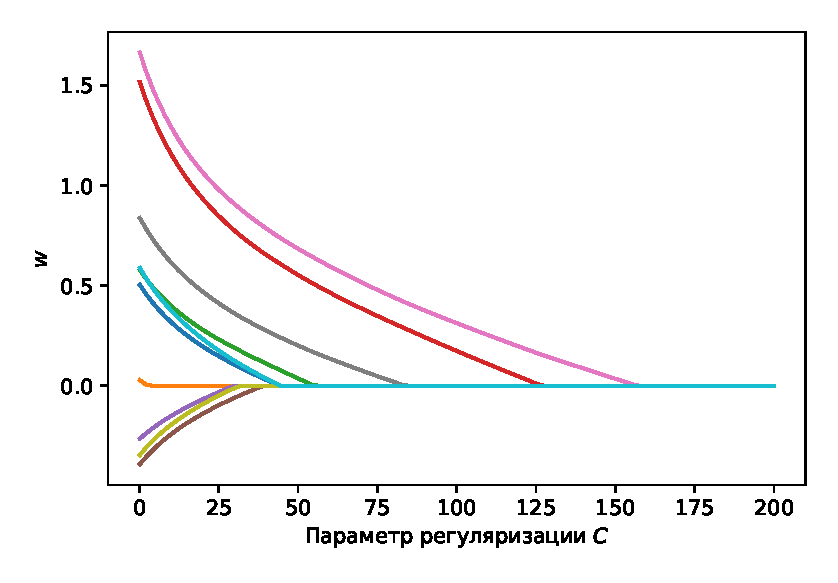
\includegraphics[width=0.5\textwidth]{../figures/log_reg_cs_exp.eps}
% 	\caption{Sample figure caption.}
% 	\label{fig:fig1}
% \end{figure}

% \subsection{Tables}
% See awesome Table~\ref{tab:table}.

% The documentation for \verb+booktabs+ (`Publication quality tables in LaTeX') is available from:
% \begin{center}
% 	\url{https://www.ctan.org/pkg/booktabs}
% \end{center}


% \begin{table}
% 	\caption{Sample table title}
% 	\centering
% 	\begin{tabular}{lll}
% 		\toprule
% 		\multicolumn{2}{c}{Part}                   \\
% 		\cmidrule(r){1-2}
% 		Name     & Description     & Size ($\mu$m) \\
% 		\midrule
% 		Dendrite & Input terminal  & $\sim$100     \\
% 		Axon     & Output terminal & $\sim$10      \\
% 		Soma     & Cell body       & up to $10^6$  \\
% 		\bottomrule
% 	\end{tabular}
% 	\label{tab:table}
% \end{table}

% \subsection{Lists}
% \begin{itemize}
% 	\item Lorem ipsum dolor sit amet
% 	\item consectetur adipiscing elit.
% 	\item Aliquam dignissim blandit est, in dictum tortor gravida eget. In ac rutrum magna.
% \end{itemize}


\bibliographystyle{unsrtnat}
\bibliography{references}

[1] Trades, Quotes and Prices, Financial Markets Under the Microscope by Jean-Philippe Bouchaud, Julius Bonart, Jonathan Donier, Martin Gould\\

[2] Multidimensional scaling in Riemann Space\\
Joseph Woelfel, George Barnett\\

[3] Dynamic Trading with Predictable Returns and Transaction Costs\\
Nicolae Gˆarleanu, Lasse Heje Pedersen\\

[4] Quasi-periodic time series clustering for human activity recognition\\
A. V. Grabovoy, V. V. Strijov\\

[5] Extracting fundamental periods to segment biomedical signals\\
Anastasia Motrenko, Vadim Strijov\\

[6] Introduction to Probabilistic Programming\\
A. Das\\

[7] Selection of superposition of models for railway freight forecasting\\
N. D. Uvarov, M. P. Kuznetsov, A. S. Malkova, K. V. Rudakov, V. V. Strijov\\

[8] Multidimensional scaling\\
$https://dept.stat.lsa.umich.edu/~jerrick/courses/stat701/notes/mds.html$

[9] Denoising diffusion probabilistic models\\
J. Ho\\

[10] Quadratic Programming Feature Selection for Multicorrelated Signal Decoding with Partial Least Squares\\
R.V. Isachenko, V.V. Strijov\\

[11] Multi-Period Trading via Convex Optimization\\
Stephen Boyd, Enzo Busseti, Steven Diamond, Ronald N. Kahn


\end{document}